\documentclass[10pt,twocolumn,letterpaper]{article}

\usepackage{cvpr}
\usepackage{times}
\usepackage{epsfig}
\usepackage{graphicx}
\usepackage{amsmath}
\usepackage{amssymb}

% Include other packages here, before hyperref.

% If you comment hyperref and then uncomment it, you should delete
% egpaper.aux before re-running latex.  (Or just hit 'q' on the first latex
% run, let it finish, and you should be clear).
\usepackage[breaklinks=true,bookmarks=false]{hyperref}

\cvprfinalcopy 

\def\httilde{\mbox{\tt\raisebox{-.5ex}{\symbol{126}}}}

\graphicspath{ {images/} }

\setcounter{page}{1}
\begin{document}

%%%%%%%%% TITLE
\title{Spotting Distracted Drivers Using Classic CV Methods}

%%%%%%%%% Author Names
\author{Guillermo Reyes\\
{\tt\small enggreys@gmail.com}
\and
Daniel Schaefer\\
{\tt\small secondauthor@i2.org}
\and
Marc Tonsen\\
{\tt\small secondauthor@i2.org}
\and
Dominik Weber\\
{\tt\small secondauthor@i2.org}
}

\maketitle

%%%%%%%%% ABSTRACT
\begin{abstract}
   The ABSTRACT is to be in fully-justified italicized text, at the top
   of the left-hand column, below the author 
   information. Use the word ``Abstract'' as the title, in 12-point
   Times, boldface type, centered relative to the column, initially
   capitalized. The abstract is to be in 10-point, single-spaced type.
   Leave two blank lines after the Abstract, then begin the main text.
\end{abstract}

%%%%%%%%% BODY TEXT

\section{Introduction}
According to the U.S. Department of Transoprtation and National Highway Traffic Safety Administration, about 18\% of all injury crashes and 10\% of fatal crashes are reported to involve distracted drivers at the moment of the accident ~\cite{knuthwebsite}. This, unfortunately, translates to over 3000 people killed and 400,000 injured per year, in the United States alone due to motor vehicle crashes.\\
This clearly speaks for measures to be taken. Spotting distracted drivers in time could help to take appropriate actions and thus prevent accidents and save thousands of lives each year. In order to detect distracted drivers, different approaches have been taken. However, many of them and intrusive and expensive. However by using simple cameras combined with computer vision algorithms, one can get a solution that is both cheap and non-intrusive.\\
For this task we have entered the Kaggle Competition: State Farm Distracted Driver Detection ~\cite{Kaggle}. The challenge consists of classifying images of drivers engaging in the behaviors described below.

\begin{enumerate}
	\item Safe driving
	\item Texting with right hand
	\item Talking on the phone with right hand
	\item Texting with left hand
	\item Talking on the phone with left hand
	\item Operating the radio
	\item Drinking
	\item Reaching behind
	\item Hair and makeup
	\item Talking to passenger
\end{enumerate}

The competition provides the dataset with over 2000 training images per class, 26 different drivers with diverse ethnic backgrounds, in 4 distinct cars and camera angles and distinctive lighting conditions as well as some noise in the data.

In this paper we propose different approaches to solve this task using some classic computer vision methods to find out how well they stack up against state of the art methods such Deep Neural Networks, which can already achieve up to 99\% accuracy .


\section{Related Work}



\section{Proposed Method}

\subsection{Hand-based classification}
\begin{figure}[h]
	\centering
	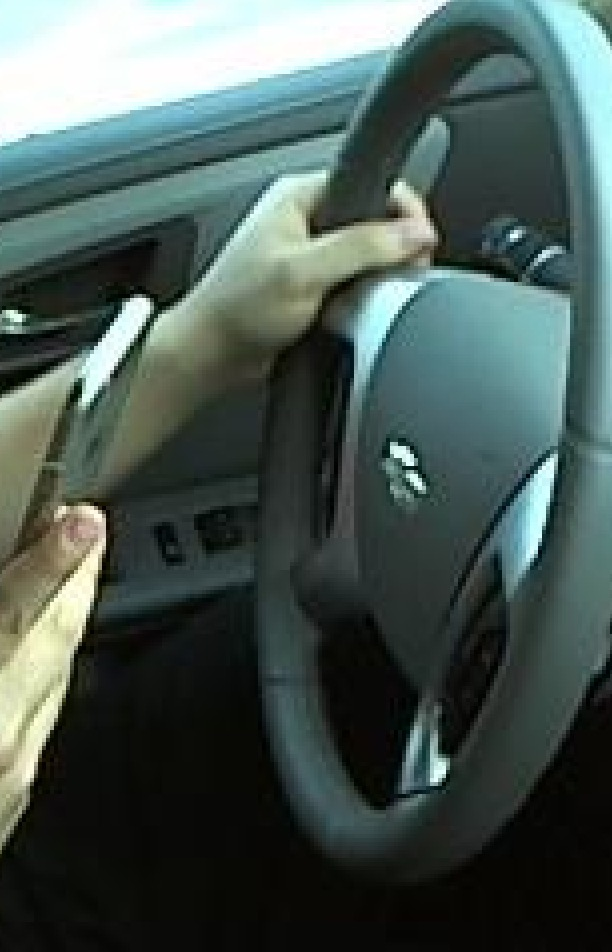
\includegraphics[width=0.2\textwidth]{handpose_example_1_cut}\hspace{0.01\textwidth}
	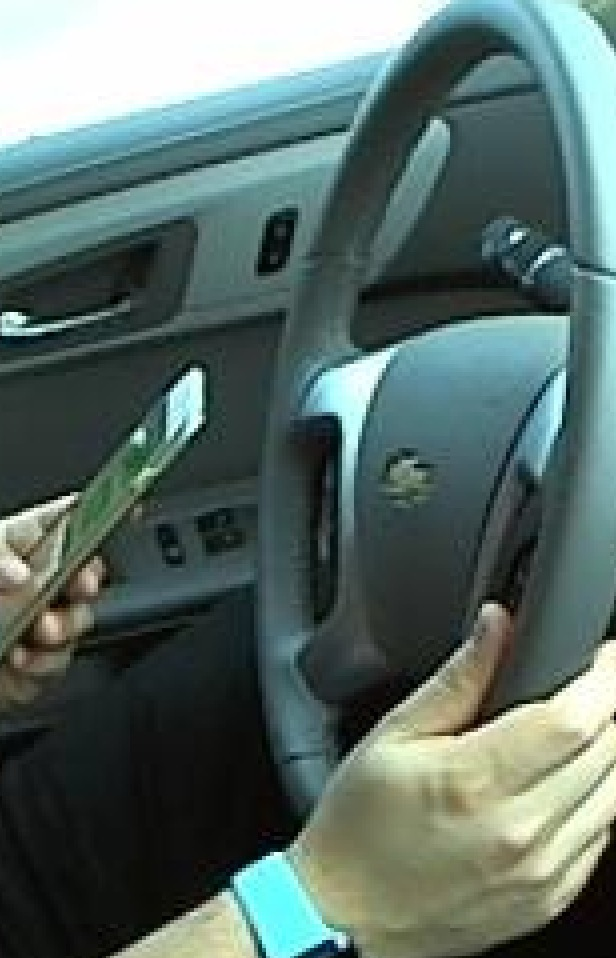
\includegraphics[width=0.2\textwidth]{handpose_example_2_cut}\\ \vspace{0.01\textwidth}
	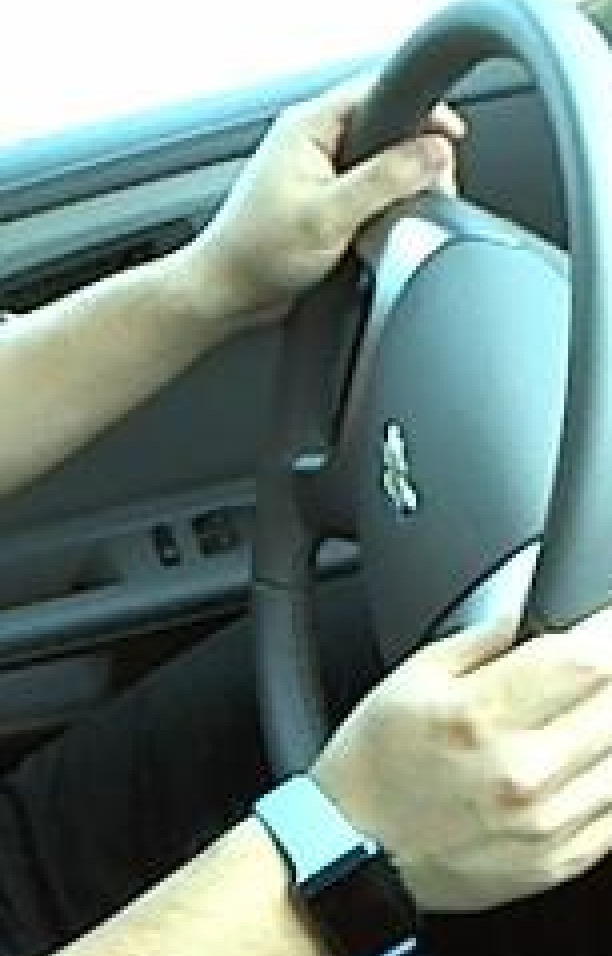
\includegraphics[width=0.2\textwidth]{handpose_example_3_cut}\hspace{0.01\textwidth}
	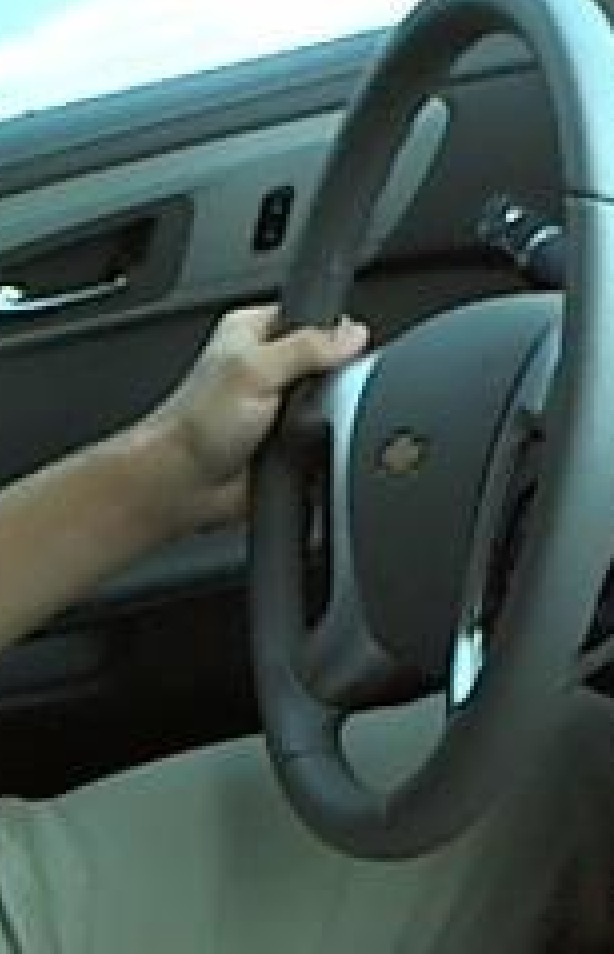
\includegraphics[width=0.2\textwidth]{handpose_example_4_cut}
	\caption{Examples of the cropped images we are using to train a classifier. The classes of the images from top-left to bottom-right are: Texting Right, Texting Left, Safe Driving, Reaching behind.}
	\label{hand_estimation_example}
\end{figure}
When examining the dataset, we found that many of the classes can be well distinguished when only considering the part of the image in the vicinity of the steering wheel. All of the activities described by the different classes in the task are performed with the arms, therefore their appearance is a strong indicator of the corresponding class. Based on this, we have cropped the images in the dataset to a fixed size of 155x240 px, to only contain the steering wheel and its immediate surroundings. See Fig. \ref{hand_estimation_example} for an illustration of those images and to see an example of how well some classes can be distinguished from that partial image. On those images we have trained a classifier to distinguish all classes and some to solve a 1-vs-1 classification task between only two classes. We have also tried to segment the classes into clusters and to classify based on those clusters, but our results were not satisfactory and we will not discuss this approach further. We have tried out different features for the classification:
\begin{itemize}
	\item \textbf{Raw Image}: We use a raw downscaled version of the image as a feature.
	\item \textbf{HoG}: Histogram of oriented gradients, which we have discussed in the lecture. We use the scikit-image implementation
	\item \textbf{LBP}: Local binary patterns, which is a feature originally developed for texture classification. It has been reported to work well in combination with HoG features in some cases. We also use the scikit-image implementation for this.
\end{itemize}
Besides using Support Vector Machines for classification, which was the only classifier discussed in the lecture, we have also tried Random Forrests.\\
It is important to note that the steering wheel is not aligned across the dataset. The training-data was recorded in 4 different cars with varying camera angles. As we will show, it is important to align the steering wheel in the cropped images for a good performance. We have manually labeled the center of all steering wheels to perform this alignment.



\subsection{HOG Landmarks}





\section{Experimental Results}

\subsection{Hand-based classification}

	\subsubsection{Alignment of the steering wheel}
	\begin{table}
		\begin{tabular}{c|c|c|c}
			& Within 1 car & No alignment & With alignment \\ 
			\hline 
			Avg. Accuracy & 37\% & 10\% & 24\% \\ 
		\end{tabular} 
		\caption{Classification accuracies for different levels of steering wheel alignment.}
		\label{hand_estimation_alignment}
	\end{table}
	
	To investigate the impact of image alignment we have trained classifiers on 3 different sets of data:
	\begin{itemize}
		\item 11 participants recorded in the same car and with the same camera angle, who are therefore perfectly aligned
		\item Unaligned crops from all participants, i.e. a window with a fixed size and position
		\item Aligned crops from all participants based on our labellings of the steering wheel
	\end{itemize}
	As one can see in Table \ref{hand_estimation_alignment} alignment significantly improves the results. The results on data coming from only a single car can be regarded as an upper limit with 37\% accuracy. With no alignment the accuracy was only 10\% which is equal to random guessing, while the accuracy was 24\% with alignment. For all further experiments the steering wheels were therefore aligned.


	\subsubsection{Feature evaluation}
	\begin{table}
		\begin{tabular}{c|c|c|c|c}
			& Raw & HoG & LBP & HoG+LBP \\ 
			\hline 
			SVR & 25\% & 32\% & 23 \% & n.A. \\ 
			\hline 
			Random Forest & 27\% & 26\% & 16\% & n.A. \\ 
		\end{tabular} 
		\caption{Classification accuracies for different features and classifiers trained on 4 participant with 1 participant for testing.}
		\label{hand_estimation_features}
	\end{table}
	Consider the classification accuracies achieved by the different combinations of features and classifiers visible in Table \ref{hand_estimation_features}. They were computed for classifiers trained on the data of 4 participants and tested on 1 participant. By far the best result was achieved with an SVM and HoG features.
	
	\subsubsection{All vs All compared to 1 vs 1}
	\begin{figure}[h]
		\centering
		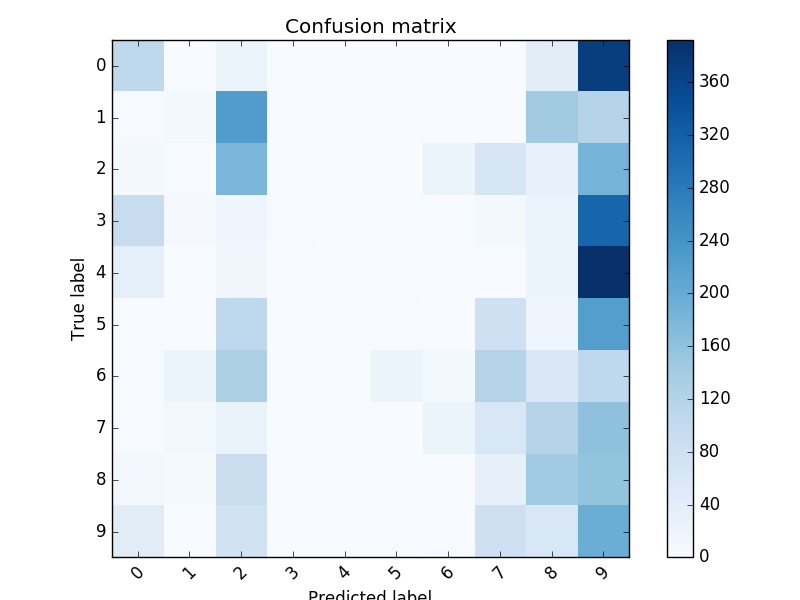
\includegraphics[width=0.5\textwidth]{handpose_plot_20p_c9}
		\caption{Confusion matrix for an SVM trained on HoG features of 20 participants (6 participants in test set).}
		\label{hand_estimation_cm}
	\end{figure}
	\begin{table}
		\begin{tabular}{c|c|c|c|c|c}
			& c1 vs c3 & c2 vs c4 & c0 vs c7 & c0 vs c5 & c3 vs c4 \\ 
			\hline 
			Accuracy & 98\% & 86\% & 94\% & 84\% & 91\% \\ 
		\end{tabular} 
		\caption{Classification accuracies for different 1-vs-1 classifiers trained on 8 participants (3 participants in test set).}
		\label{hand_estimation_1vs1}
	\end{table}
	Although the classification accuracy of an SVM with HoG features is significantly better then random with more then 30\%, it is not good enough to be practically relevant. The confusion matrix in Figure \ref{hand_estimation_cm} displays the classification errors of a classifier trained on 20 participants (6 participants in the test set) and HoG features. There does not seem to be any logically explainable confusion. To further investigate our thesis that some of the classes should be easy to distinguish based on the appearance of the hands on the steering wheel, we trained a few 1-vs-1 classifiers. As is illustrated in Table \ref{hand_estimation_1vs1}, they did achieve a very good accuracy. 
	
	
\subsection{HOG Landmarks}




\section{Conclusion}

\section{Future Work}



%%%%%%%%% REFERENCES

{\small
\bibliographystyle{ieee}
\bibliography{egbib}
}

\end{document}
